\section{Cleric Class Weapons}

\subsubsection{Chalice of Light}

The Chalice of Light is known in Legend to be a holy war hammer imbued directly with the presence of a divine spirit. It is believed that Apollo had a follower so loyal and faithful that Apollo sent an angel to reside within this particular war hammer and protect the wielder during his dangerous missionary journeys. The hammer was originally forged by a dwarven clan which dedicated themselves to Apollo. Per legend, a high priest of Apollo took it upon himself to set forth into the most dangerous lands to preach that of Apollo. Among his second journey, he found himself being ambushed and sent to his death in a place called The Undercity. In a fervent prayer, his war hammer became light to the tough, and changed it's appearance to hold an everlasting flame that burned alongside his faith and gave the high priest the ability to break free from his bonds and purge The Undercity of the sins that corrupted it and the surrounding lands. The flame of the burning hammer is said to have ceased when the wielder died of old age. It is believed that if the hammer is found, it is already forged to hold the essence of an angel and can provide uncanny abilities to a man of great faith.

\begin{center}
	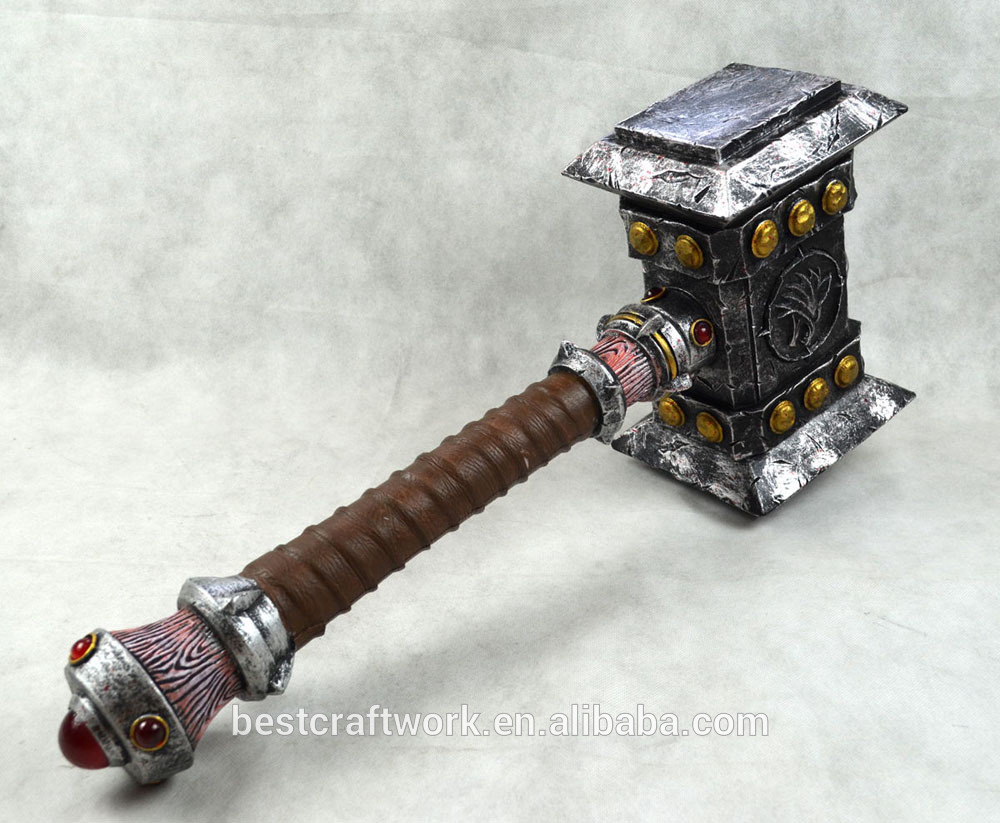
\includegraphics[width=0.41\linewidth]{img/weapons/Wow-Hammer.jpg} 	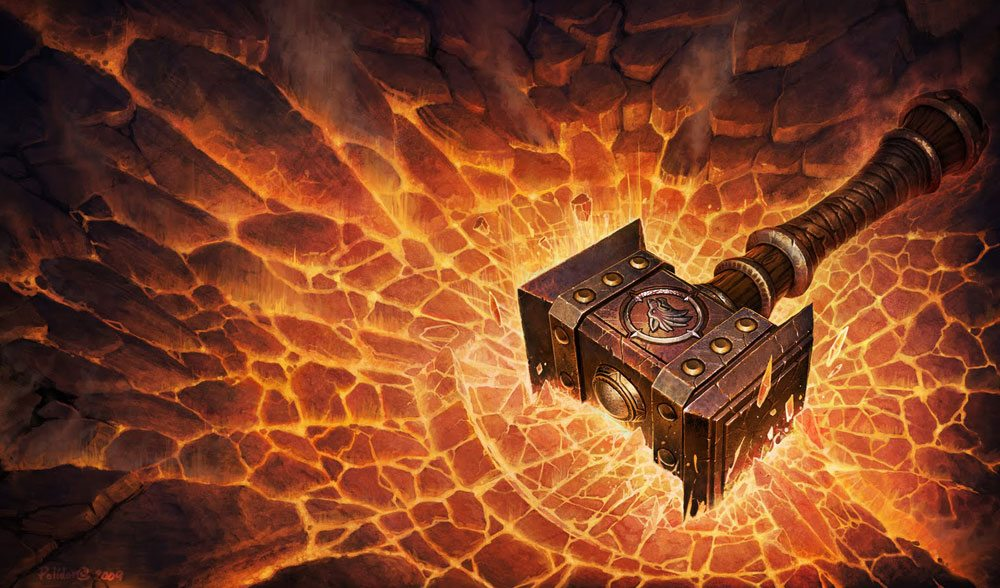
\includegraphics[width=0.57\linewidth]{img/weapons/shatteredhand.jpg}
\end{center}

\subsubsection{Potential}

The Chalice of Light weapon wants to be wielded by a religious character. 

\begin{commentbox}{Chalice of Light\footnote{Weapon (war hammer), artifact (requires attunement by a cleric)}}   
	If no angel or spirit from a deity is with this weapon, it is a simple warhammer that only does 1d8 bludgeoning damage.
	
	You gain a +3 bonus to attack and damage rolls made with this magic weapon. When you hit an enemy you will deal 1d6 fire damage and 1d6 radiant damage. The damage will change to d10's if the target rejects the clerics deity (they must know of them though).
	
	When you take damage while wielding the Chalice of Light, you can heal one target within 50 yards for a single roll of the dice closes to the wielders level (round up).
	
	While a cleric wields The Chalice of Light in combat it will look like the cleric is burning with a holy flame. Anyone who rejects the clerics deity that attacks the wielder will take 1d6 fire damage and 1d6 radiant damage. When the wielder rolls a 20 against someone who rejects their deity, a wielder must a d100 roll. If the roll is less than half the wielders lvl then the attacker will burn in holy flame and turn to ash immediately.
	
	If a cleric of an evil alignment tries to attune to The Chalice of Light they have to make a d20 roll. At a 18 or below The Chalice of Light will reject you and deal 3d10 fire damage and 2d10 radiant damage. At a 19 or 20 you over power the will of the weapon and make it yours.
	
	With a successful roll to overcome the will of The Chalice of Light while having an evil alignment will make The Chalice of Light's appearance will start to dull and become darker until it becomes fully corrupt. It will regain its former glory when its attuned to a cleric of a non evil alignment.
	
	Proficiency with a war hammer allows you to add your proficiency bonus to the attack roll for any attack you make with it.
	
	If the wielder of Chalice of Light dies (by failing three death saves) then the angel within the hammer can leave the weapon and resurrect the player to full. The weapon after this point becomes useless.
\end{commentbox}


\subsubsection{Finding the Chalice of Light}

